%%%%%%%%%%%%%%%%%%%%%%%%%%%%%%%%%%%%%%%%%%%%%%%%%%%%%%%%%%%%%%%%%%%%%%%%%%%%%%%%%
%																				%
%	TRABAJO:	Trabajo Final													%
%				Especialidad en Ingenier�a en Sistemas de Informaci�n			%
%																				%
%		Titulo:																	%
%																				%
%		Autores:	Julian Nonino												%
%																				%
%	Capitulo sobre Apache Flink													%	
%																				%
%	A�o: 2016																	%
%																				%
%%%%%%%%%%%%%%%%%%%%%%%%%%%%%%%%%%%%%%%%%%%%%%%%%%%%%%%%%%%%%%%%%%%%%%%%%%%%%%%%%

\chapter{Apache Flink}
\label{chapter_apache_flink}



\section{Conceptos\cite{ApacheFlink10Docs}}

	Los \emph{programas Flink} son programas comunes que implementan
	transformaciones en colecciones distribuidas, por ejemplo, filtrado,
	correspondencia, actualizaci�n de estado, uniones, agrupamientos, agregaciones,
	etc�tera. �stas colecciones se forman a partir de las fuentes de datos
	(\emph{sources}). Dichas fuentes se forman leyendo archivos, conectando Flink a
	un servidor de mensajes como Apache Kafka \ref{chapter_apache_kafka} o mediante
	colecciones definidas localmente.
	
	Los resultados de la ejecuci�n de un programa Flink son devueltos mediante el
	uso de receptores de datos \emph{sinks}. �stos receptores pueden consistir en
	escritura de archivos, impresi�n en la consola de ejecuci�n, etc�tera.
	
	Los programas Flink pueden correr localmente (standalone), embebidos en otros
	programas o en clusters.
	
	Dependiendo del tipo de fuente de datos (\emph{source}), es decir, acotados o
	no acotados, el programa Flink deber� realizar una ejecuci�n por lotes
	(\emph{batch}) o una ejecuci�n en tiempo real sobre el flujo de datos
	(\emph{straming}). Para el primer caso, se deber� utilizar la
	\textbf{\emph{DataSet API}} y para el segundo caso la \textbf{\emph{DataStream
	API}}.
	
	Los bloques b�sicos de un programa Flink son los flujos de datos (streams) y
	las transformaciones (operaciones).

	Al ejecutarse, un programa Flink se corresponde con lo que se conoce como
	\emph{Streaming Dataflow}. Cada \emph{Dataflow}, comienza con una o m�s fuentes
	de datos (\emph{sources}) y termina en uno o m�s receptores de datos
	(\emph{sinks}).
	En la mayor�a de los casos, existe una correspondencia uno a uno entre las
	transformaciones especificadas en el programa y las operaciones del
	\emph{Dataflow} pero puede ocurrir que una transformaci�n est� formada por mas
	de un operador de transformaci�n.
	
	\begin{figure}[H]
		\centering
		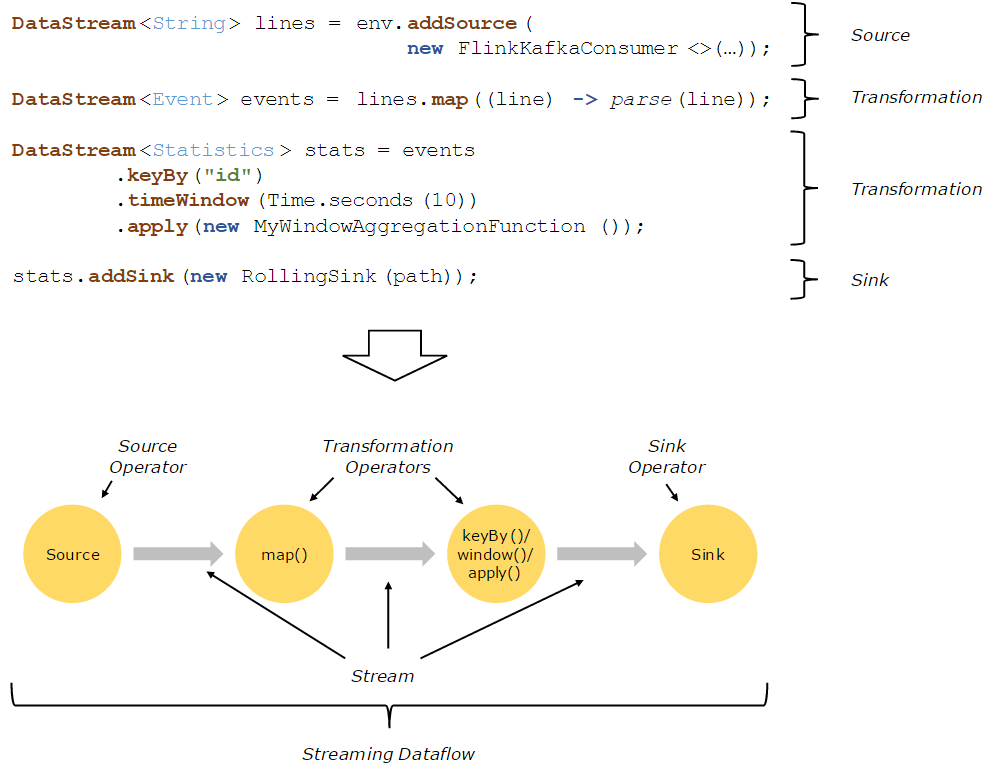
\includegraphics[width=1\linewidth]{./marco_teorico/img/flink/building_blocks}
		\caption{Bloques Fundamentales de un Programa Flink\cite{ApacheFlink10Docs}}
	\end{figure}

\subsection{Usar Flink}
	
		Para escribir un programa Flink, se deben incluir las libre�as Flink en el
		proyecto, en el caso de Maven, �sto se logra insertando las siguientes l�neas
		en el pom.xml del proyecto.
		
\lstset{language=XML}
\begin{lstlisting}
<dependency>
	<groupId>org.apache.flink</groupId>
	<artifactId>flink-core_2.11</artifactId>
	<version>1.0.3</version>
</dependency>
<dependency>
	<groupId>org.apache.flink</groupId>
	<artifactId>flink-java_2.11</artifactId>
	<version>1.0.3</version>
</dependency>
<dependency>
	<groupId>org.apache.flink</groupId>
	<artifactId>flink-clients_2.11</artifactId>
	<version>1.0.3</version>
</dependency>
<dependency>
	<groupId>org.apache.flink</groupId>
	<artifactId>flink-streaming-java_2.11</artifactId>
	<version>1.0.3</version>
</dependency>
<dependency>
	<groupId>org.apache.flink</groupId>
	<artifactId>flink-connector-kafka-0.9_2.11</artifactId>
	<version>1.0.3</version>
</dependency>
\end{lstlisting}
	
	\subsection{DataSet y DataStreams\cite{ApacheFlink10Docs}}		

		Para representar datos en un programa Flink existen dos tipos de clases
		DataSet y DataStream. Se puede considerar que son colecciones inmutables de
		datos que pueden contener duplicados. En el caso del DataSet la cantidad de
		datos es finita, mientras que en un DataStream pueden ser ilimitados.
		
		�stas colecciones son diferentes a las Java en el sentido de que son
		inmutables, una vez creadas no pueden a�adirse ni removerse elementos. Tampoco
		es posible inspeccionar los elementos contenidos dentro de la colecci�n.
		
		Como se menciono anteriormente, una colecci�n DataSet o DataStream es creada
		en el momento en que se a�ade una fuente de datos \emph{source} y nuevas
		colecciones son creadas cada vez que una operaci�n de transformaci�n es
		ejecutada.

	\subsection{Evaluaci�n Postergada}
	
		Al ejecutar un programa Flink, el m�todo \emph{main} es ejecutado pero la
		carga de datos y las transformaciones no ocurren directamente. Cada operaci�n
		es creada y a�adida a un plan de ejecuci�n del programa. Las operaciones, son
		ejecutadas cuando son exlicitamente disparada mediante el llamado del m�todo
		\emph{execute()} sobre el entorno de ejecuci�n \cite{ApacheFlink10Docs}.


\section{Flink DataStreams}

API Programming Guide (Source: https://ci.apache.org/projects/flink/flink-docs-release-1.0/apis/streaming/index.html)

DataStream programs in Flink are regular programs that implement transformations
on data streams (e.g., filtering, updating state, defining windows,
aggregating). The data streams are initially created from various sources (e.g.,
message queues, socket streams, files). Results are returned via sinks, which
may for example write the data to files, or to standard output (for example the
command line terminal). Flink programs run in a variety of contexts, standalone,
or embedded in other programs. The execution can happen in a local JVM, or on
clusters of many machines.


\section{Material}

	La informaci�n de �ste cap�tulo ha sido extra�da mayormente desde la
	documentaci�n de Apache Flink 1.0 \cite{ApacheFlink10Docs}.
